

This stone is mostly inspired by Kellogg \& King (1997) \cite{keki97}. 

\begin{center}
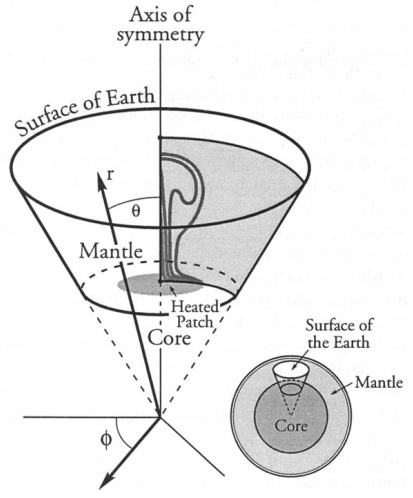
\includegraphics[width=5cm]{python_codes/fieldstone_106/images/keki97a}\\
{\captionfont Taken from \cite{keki97}.}
\end{center}
The Rayleigh number is defined by
\[
\Ranb 
= \frac{\rho_0 g \alpha \Delta T (R_{outer}-R_{inner})^3}{\eta_0 \kappa}
=\frac{\rho_0^2 C_p g \alpha \Delta T (R_{outer}-R_{inner})^3}{\eta_0 k}
\]
The original article relies on dimensionless mass, momentum and energy conservation equations
but does not provide enough information to attempt an identical replication. I therefore 
choose here parameters which yield the same Rayleigh number $\Ranb=10^7$:
\begin{itemize}
\item $\rho_0=3300\si{\kg\per\cubic\metre}$
\item $\alpha=3\cdot 10^{-5} \si{\per\kelvin}$
\item $\Delta T=3000\si{\kelvin}$
\item $R_{inner}=3480\si{\km}$
\item $R_{outer}=6371\si{\km}$
\item $k=3$
\item $C_p=1250$
\item $g=9.81\si{\metre\per\square\second}$
\end{itemize}
The viscosity is then 
\[
\eta_0
=\frac{\rho_0^2 C_p g \alpha \Delta T (R_{outer}-R_{inner})^3}{\Ranb k}
\simeq 9.66 \cdot 10^{21}\si{\pascal\second}
\]
The domain is a section of an annulus with an angular opening of $\pi/4$. 
It is centered around the vertical axis. 



The viscosity is either constant ($\eta_0$) or temperature-dependent 
\[
\eta(T')
=\eta_0 \exp\left[ \frac{E}{R \Delta T} \left( \frac{1}{T'+t_0} -\frac{1}{1+t_0}  \right)   \right]
=\eta_0 \exp\left[ \frac{E}{R} \left( \frac{1}{T' \Delta T  +t_0 \Delta T} -\frac{1}{\Delta T +t_0 \Delta T}  \right)   \right]
\]
where ``$t_0$ is the surface temperature $T_{surf}$ divided by 
the temperature drop across the shell $\Delta T$'', and 
I think the authors took 
\[
T'=\frac{T-T_s}{T_p-T_s}= \frac{T-T_s}{\Delta T}
\]
\[
\eta(T)
=\eta_0 \exp\left[ \frac{E}{R} \left( \frac{1}{T-T_s  + T_s} -\frac{1}{T_p-T_s + T_s}  \right)   \right]
=\eta_0 \exp\left[ \frac{E}{R} \left( \frac{1}{T} -\frac{1}{T_p}  \right)   \right]
\]
so that $\eta(T_p)=\eta_0$. 
The authors investigate three cases:
\[
\frac{E}{R \Delta T} = \{0,0.25328,3\}
\]
With $R=8.31$ and $\Delta T=3000$ then $E=\{ 0, 6317.6 , 74829.6 \}$.
As in the paper, the viscosity is ``clipped'' to $1000\eta_0$.

\begin{remark}
At the moment the code is 2D, not axisymmetric! Also, the side walls are no-slip, 
not free slip. I had to guess the size of the patch as it is not specified in the paper.
LK filter and/or SUPG should be tested (at the moment the temperature us thresholded in the 
material model). Explore resolution, initial T in the mantle, try Steinberger average 
viscosity profile, look at dynamic topography, strain-rate dependent power-law rheology, ...
I think it would nake more sense to use Tmantle in the rheology than Tpatch. All models would then start
with the same viscosity in the mantle, only thermal boundaries would have viscous variations.
\end{remark}


%%%%%%%%%%%%%%%%%%%%%%%%%%%%%%%%%%%%%%%%%%%%%%%%%%%
\subsubsection*{Isoviscous model}
\begin{center}
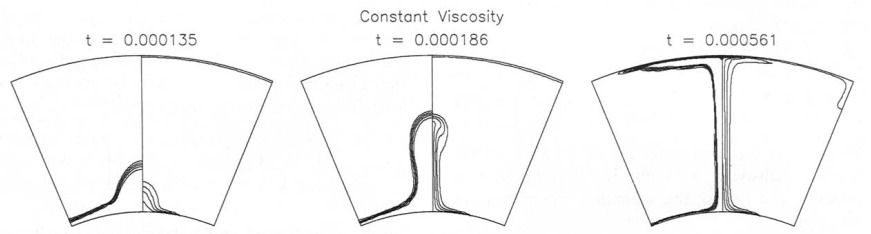
\includegraphics[width=15cm]{python_codes/fieldstone_106/images/keki97b}
\end{center}

%%%%%%%%%%%%%%%%%%%%%%%%%%%%%%%%%%%%%%%%%%%%%%%%%%%
\subsubsection*{Weakly temperature-dependent model}
\begin{center}
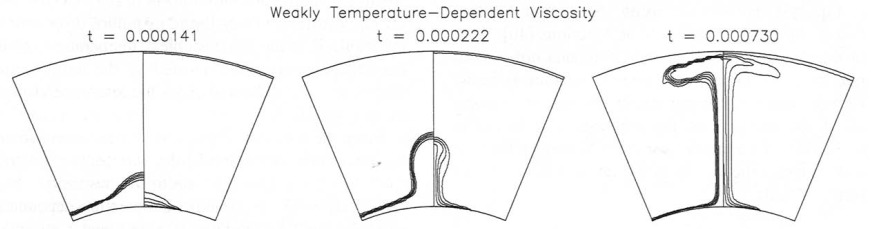
\includegraphics[width=15cm]{python_codes/fieldstone_106/images/keki97c}
\end{center}

%%%%%%%%%%%%%%%%%%%%%%%%%%%%%%%%%%%%%%%%%%%%%%%%%%%
\subsubsection*{Strongly temperature-dependent model}
\begin{center}
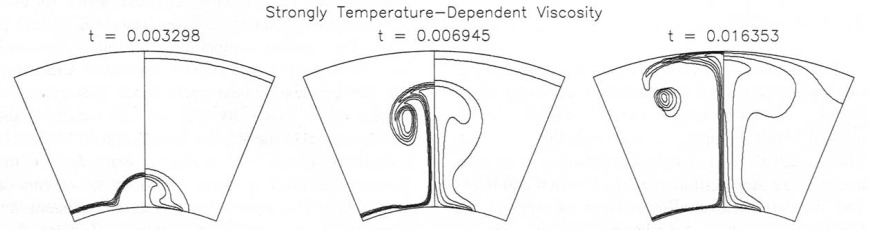
\includegraphics[width=15cm]{python_codes/fieldstone_106/images/keki97d}
\end{center}



